\chapter{Requirements}
\section{Book search app}
\textsc{Book Search App} is a simple Android app that leverages the OpenLibrary API (\url{https://openlibrary.org/developers/api}) to search books and display cover images and basic information about them. It is possible to download and install the application on a device from the following link: \url{http://softeng.polito.it/courses/01GSP/booksearch.apk}.

\paragraph{Stakeholder analysis}
\begin{itemize}
\item End user;
\item Developer;
\item Other developers downloading app from GitHub to extend/modify it;
\item Possibly Open Library developers.
\end{itemize}
There is no administrator, because there is no database. The end user is the administrator of his/her own mobile phone.

Open Library is a passive actor which receives queries and responds to them.

\paragraph{Context diagram} See table~\ref{tab:book_context}. The key information of the context diagram is that the collection of book descriptors is \emph{outside} the scope of the app.

\begin{table}
\centering
\footnotesize
\begin{tabular}{|l|l|l|}
\hline
\textbf{Actor} & \textbf{Physical interface} & \textbf{Logical interface} \\
\hline
End user & Smartphone (touchscreen, buttons) & GUI (2 or 3 screens) \\
\hline
Open Library & Internet connection & Open Library API \\
\hline
Android intent framework & Smartphone & Android intent API \\
\hline
\end{tabular}
\caption{Context diagram}
\label{tab:book_context}
\end{table}

\paragraph{Functional requirements} See table~\ref{tab:book_functional}.
\begin{table}
\centering
\small
\begin{tabularx}{\textwidth}{|l|X|}
\hline
\textbf{Req. ID} & \textbf{Description} \\
\hline
FR1 & Search book given string of text (will match with any book descriptor field) in Open Library \\
\hline
FR2 & Show results of search (show many book descriptor with little detail) \\
\hline
FR3 & Share book descriptor with other applications on Android \\
\hline
FR4 & Show one book descriptor in full detail (all fields and cover picture) \\
\hline
FR5 & The app should work also in case of no internet connection (no results in case of FR1, but no crash happens) \\
\hline
\end{tabularx}
\caption{Functional requirements}
\label{tab:book_functional}
\end{table}

\paragraph{Non functional requirements} See table~\ref{tab:book_nonfunctional}.

\begin{table}
\centering
\small
\begin{tabularx}{\textwidth}{|l|l|X|}
\hline
\textbf{Req. ID} & \textbf{Type} & \textbf{Description} \\
\hline
NF1 & Usability & Average smartphone user (uses a smartphone every day since at least one year, using at least one app per day) should be able to use the application in less than 5 minutes \\
\hline
NF2 & Performance (speed) & Functions FR2 to FR4 should complete in less than 0.5 sec. FR1 should complete in less than 0.5 sec excluding network and Open Library delays \\
\hline
NF3 & Performance (space) & The app should use less than 100~MB RAM and 10~MB disk \\
\hline
NF4 & Portability & The app should run on all Android versions from 3.0 \\
\hline
NF5 & Privacy & The app should not disclose any information about the user or smartphone where is is installed \\
\hline
NF6 & Reliability & Out of 1000 usages of the app, the app should crash at most once \\
\hline
\end{tabularx}
\caption{Non functional requirements}
\label{tab:book_nonfunctional}
\end{table}

\paragraph{Use cases}
See table~\ref{tab:book_usecases} and figure~\ref{img:book_context}.
\begin{table}
\begin{tabularx}{\textwidth}{|l|X|X|X|}
\hline
\textbf{Actor} & \textbf{Goal} & \textbf{Description} & \textbf{Scenario ID} \\
\hline
End user & Search books given string of text & Search book descriptors that match the vgiven string on any field of the book descriptor & Scenario 1, Scenario 2, Scenario 3 \\
\hline
End user & Share book descriptor with other app on smartphone & Having selected a book descriptor, the search app shares it with another app using Android intents & Scenario 4 \\
\hline
\end{tabularx}
\caption{Use cases}
\label{tab:book_usecases}
\end{table}

\begin{figure}[hbtp]
\centering
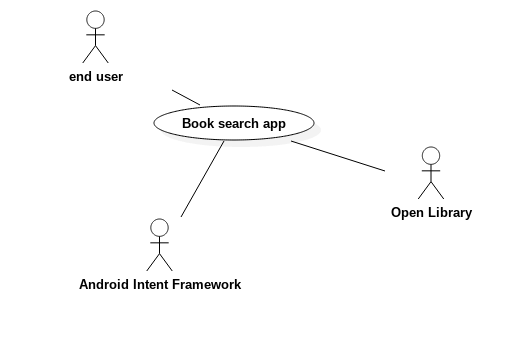
\includegraphics[scale=0.45]{exercises/book_contextDiagram.png}
\caption{Book search app - Context diagram}
\label{img:book_context}
\end{figure}

\subparagraph{Scenario}
Some scenarios are listed in tables~\ref{tab:scenario1}, \ref{tab:scenario2}, \ref{tab:scenario3} and \ref{tab:scenario4}.

\begin{table}
\small
\begin{tabularx}{\textwidth}{|l|X|l|}
\hline
\textbf{Step} & \textbf{Action} & \textbf{Req. ID} \\
\hline
1 & User writes a string of text & \\
\hline
2 & App sends request to Open Library, retrieves results & FR1 \\
\hline
3 & App shows results on screen & FR2 \\
\hline
\end{tabularx}
\caption{Scenario 1}
\label{tab:scenario1}

\begin{tabularx}{\textwidth}{|l|X|l|}
\hline
\textbf{Step} & \textbf{Action} & \textbf{Req. ID} \\
\hline
1 & User writes a string of text & \\
\hline
2 & App sends request to Open Library, retrieves results & FR1 \\
\hline
3 & No results, app shows `No match' message on screen & FR2 \\
\hline
\end{tabularx}
\caption{Scenario 2}
\label{tab:scenario2}

\begin{tabularx}{\textwidth}{|l|X|l|}
\multicolumn{3}{l}{Precondition: end user has installed the app, has internet connection working.} \\
\multicolumn{3}{l}{Postcondition: no result shown to end user.} \\
\hline
\textbf{Step} & \textbf{Action} & \textbf{Req. ID} \\
\hline
1 & User writes a string of text & \\
\hline
2 & App sends request to Open Library, retrieves results & FR1 \\
\hline
3 & More than 100 results, app shows `Too many matches' message on screen & FR2 \\
\hline
\end{tabularx}
\caption{Scenario 3}
\label{tab:scenario3}

\begin{tabularx}{\textwidth}{|l|X|l|}
\multicolumn{3}{l}{Precondition: end user has performed a search and selected book descriptor B.} \\\multicolumn{3}{l}{Postcondition: the application A, selected by the user, has received B.} \\
\hline
\textbf{Step} & \textbf{Action} & \textbf{Req. ID} \\
\hline
1 & End user requests to share B & \\
\hline
2 & App passes B information to Android intent & FR3 \\
\hline
3 & End user selects other application A to share information with & \\
\hline
4 & Android intent passes B to A & \\
\hline
\end{tabularx}
\caption{Scenario 4}
\label{tab:scenario4}
\end{table}

\paragraph{Glossary}
See figure~\ref{img:book_glossary}. End user is not a class because there is no need of track a user, i.e.,\@ no username, no login, no logout, \dots

\begin{figure}[hbtp]
\centering
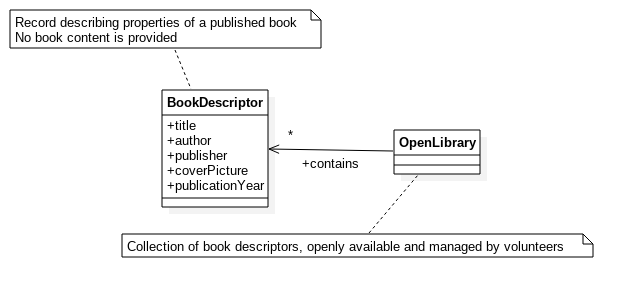
\includegraphics[scale=0.45]{exercises/book_glossary.png}
\caption{Book search app - Glossary}
\label{img:book_glossary}
\end{figure}